\chapter{Konzept}
In diesem Kapitel wird das in diesem Bericht genutzte Konzept beschrieben. Das Grundkonzept bestehet darin, dass der zu befahrene Bereich in einen Fertigungsbereich und einen Transportbereich unterteilt wird. Die Grenzen der Bereiche sind in Abbildung \ref{fig:Bereiche} dargestellt. Im Transportbereich, in der Abbildung \ref{fig:Bereich} nicht eingefärbt, wird die Regelung des Robotinos über die Potentialfeldmethode realisiert. Das dabei genutzte Potentialfeld wird unter Kapitel \ref{sec:Potential} näher erläutert. Im Fertigungsbereich wird die Regelung von der Bahnregelungsgruppe übernommen. Um zwischen den Bereichen zu wechseln, werden Übergabepunkte definiert, an denen der Bereichswechsel sicher ausgeführt werden kann. Diese Übergabepunkte sind in der Abbildung als rote Kreise dargestellt. Dazu wird eine Kommunikation zwischen den Einzelgruppen über eine Schnittstelle definiert. Diese Schnittstelle wird in Kapitel \ref{} definiert. Desweiteren wird das Konzept zum Vermeiden von Kollisionen in Kapitel \ref{} näher beschrieben. Dabei wird auf verschiedene Hindernistypen eingegangen. Um das Konzept abzuschließen wird in Kapitel \ref{} der Ablauf des Programmes dargestellt.

\begin{figure}[!h]
	\centering	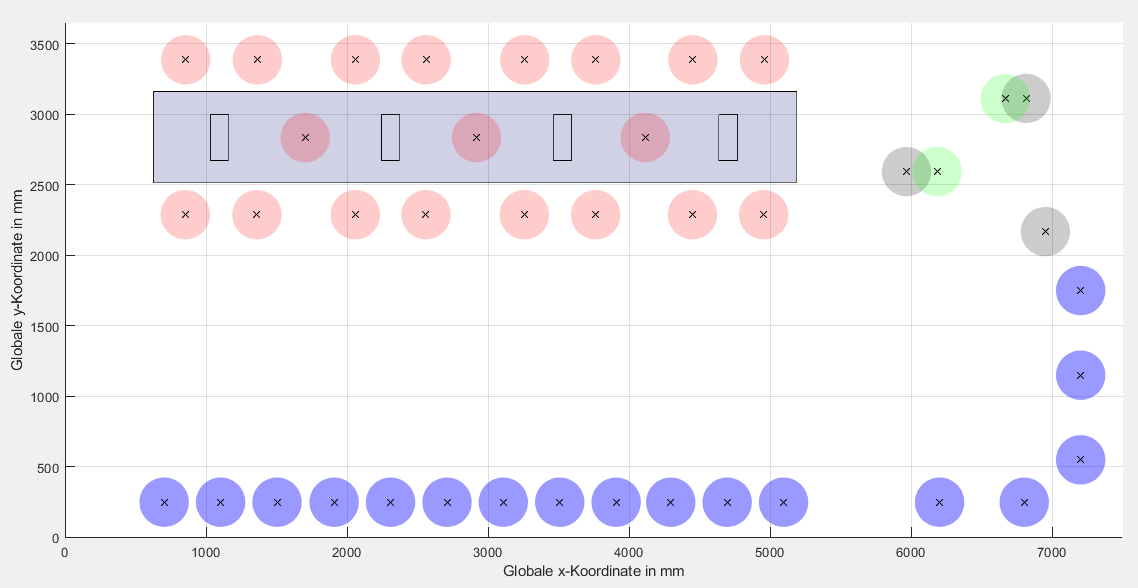
\includegraphics[width=0.8\textwidth]{grafiken/TransportbereichKarte.png}
	\caption{Bereichseinteilung}
	\label{fig:Bereiche}
\end{figure}